\documentclass{article}
\usepackage[utf8]{inputenc}
\usepackage{graphicx}
\usepackage{lipsum}
\usepackage{float}
\usepackage[margin=1in,left=1.5in,includefoot]{geometry}

% Header and Footer
\usepackage{fancyhdr}
\pagestyle{fancy}
\fancyhead{}
\fancyfoot{}
\fancyfoot[R]{ \thepage\ }
\renewcommand{\footrulewidth}{0pt}
%


\begin{document}

% title page content
\begin{titlepage}
    \begin{center}
        
\includegraphics[height= 4cm ]{UoRlogo.png} \\
        [5mm]
        \textsc{\Large University of Reading} \\
        [0.5cm]
        \textsc{\Large Department of Computer Science} \\
        [1cm]

        \line(1,0){300}\\
        [0.25in]
        \huge{\bfseries Extending a Platform Game in C/CC++: User Experience Enhancement}\\
        [2mm]
        \line(1,0){200} \\
        [1cm]
        \textsc{\Large Jason Jay Dookarun} \\
        [2mm]
        \textsc{\large Word Count: TBC} \\
        [2mm]
        \textsc{\large Page Count: 6}\\
        [4cm]
        \end{center}
        \begin{flushright}
        \textsc{\normalsize Module Code: CS1PR16 \\
        Assignment Report Title: Programming Project \\
        Student Number: 26017434 \\
        Time Spent: 50 Hours \\
        April 21, 2020 } \\
        \end{flushright}
\end{titlepage}

% front matter
\pagenumbering{roman}
\section*{Summary}
\addcontentsline{toc}{section}{\numberline{}Summary}

The following document consists of an in-depth systematic examination of elements developed by I, Jason Jay Dookarun, to an existing C/C++ program developed by Parallel Realities. The given program is a platform game that employs the SDL2 library for the demonstration of graphics. A feature has been composed, modified and extended, integrated within the provided game, with the support provided by the skeleton code, authorised by \textbf{Dr Julian Krunkel} of the Department of Computer Science at the University of Reading. The aforementioned will further elaborate on the procedures undertaken to develop the feature(s) including design illustrations, methods of implementation and development process.

\section*{Declaration}
\addcontentsline{toc}{section}{\numberline{}Declaration}

I, \textbf{Jason Jay Dookarun}, of the Department of Computer Science at the University of Reading, confirms that all the sentences, figures, tables, equations, code snippets, artwork and illustrations in this report are original and have not been taken from any other person’s work, except where the works of others have been explicitly acknowledged, quoted and referenced. I understand that if failing to do so will be considered as a case of plagiarism. Plagiarism is a form of academic misconduct and will be penalised accordingly.

    \begin{flushright}
    \textbf{Jason Jay Dookarun} \\
    April 21, 2020\\
    [1cm]
    \end{flushright}

%\cleardoublepage
\tableofcontents
\thispagestyle{empty}
%\cleardoublepage

\listoffigures
\addcontentsline{toc}{section}{\numberline{}List of Figures}
\cleardoublepage





\newpage
\section{Introduction}\label{sec:intro}
\rhead{Introduction}
\lhead{Extending a Program in C/C++}
The provided program employs an SDL2 library to illustrate graphical components, coded in C/C++. This program has been developed and created by Parallel Realities. This project aims to develop an extension to the existing piece and further describe the choice made and implementation cycle applied. Authorised by the academic staff members at the University of Reading, I was provided with a skeleton code containing sections of the existing platform game, namely "Pete's Pizza Party 6".

The aim of the game entails accumulating all objects positioned across disparate seconds of the map. These objects would be portrayed as pizza slices. As the user assembled every pizza slice, the HUD, located on the right-hand side of the user's screen, would increment, accordingly. Once the entity collected all the elements, the game would be terminated.

To understand the game and existing mechanisms implemented, my first initiative involved executing the program. This allowed me the remark sectors of the program that could be: added, improved or modified. Moreover, by applying such, I would then be able to understand what sections of the game could be either improved or added, by using previous knowledge of gaming.
\begin{figure}[H]
    \centering
    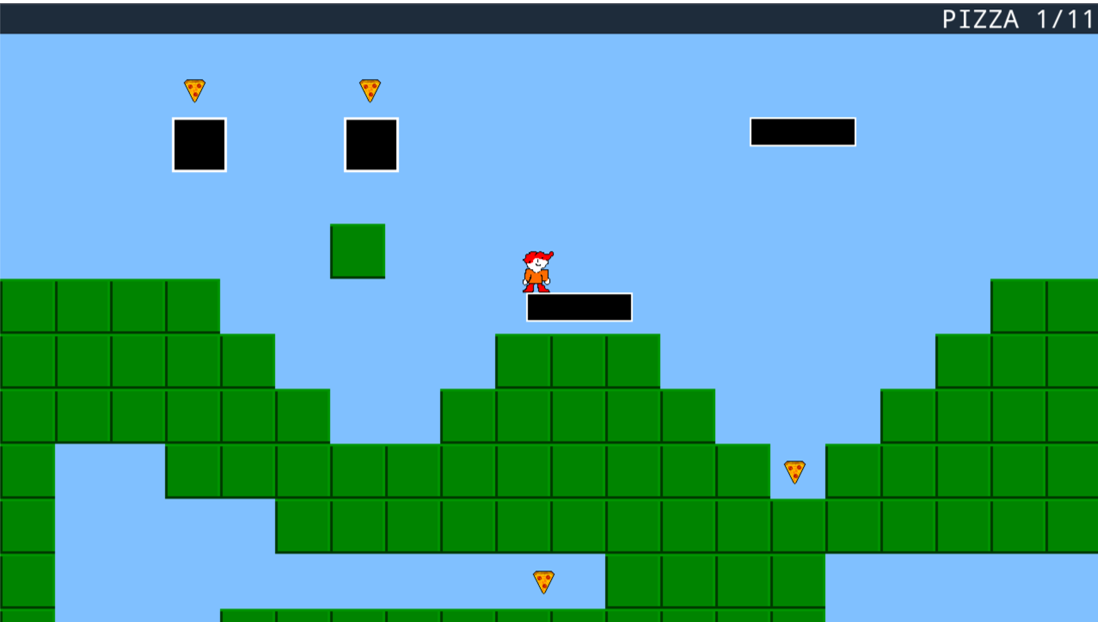
\includegraphics[height=3in]{figure1.png}
    \caption[Pete's Pizza Party: Pre-Extension]{Pete's Pizza Party: Pre-Extension}
    \label{fig:pete's pizza party}
\end{figure}
Figure \ref{fig:pete's pizza party} illustrates one of the first instances of running the aforementioned.
After running several instances, I was able to identify numerous components that could've been adjusted or implemented to provide the user with enhanced user experience, namely universal control commands, a support panel and an introduction sequence to allow the user to comprehend the product.

User experience can be characterised as a "quality attribute of the UI, covering whether the system is easy to learn, efficient, pleasant, and so forth". \cite{userexperience} Conclusively, user experience can be adopted as a way of testing, to perceive whether a product warrants a positive user experience. To ensure such is achieved, I decided to use the aforementioned as guidance when executing the program.

Currently, the product implements any player movement the use of the letters A, D, I and SPACE, where A represents a movement to the left, D represents a movement to the right, I represents jump, and SPACE represents a reset functionality. This could be potentially identified as a difficulty for the user, as a universal control panel is not implemented. Moreover, no support is provided to the user for one to understand what the controls may be. This sector can, as a result, be identified as a weakness, allowing such an extension to be provided.


Moreover, once the program is executed, the user is immediately provided with the main program. As a result, the user is not provided with a formal welcome to the game and intricately links to the avoidance of positive user experience. Furthermore, once the user does complete collecting all objects displayed on the map, the user is not provided with an option to play again, but instead is forced to view the game terminated. Both of the raised weaknesses interlink with the subject of user experience, as both consequently do not fulfil positive UX (User Experience) for the user. This, as a consequence, provided me with a segment to converge upon, to transform and intensify the product for future clientele.




\section{Design}\label{sec:design}
Following my brief analysis of the program before development, I believe that it would be useful to focus on changes correlating to one's perception of the user's experience. This would include an introduction to the main splash screen to welcome the user, implementing a support page within the main screen, and further support during live game-play. Further, controls are to be also modified to implement a universal control scheme for ease of use. Finally, a closing progression would be performed to allow the user to either: play the game again or exit the game appropriately, as an alternative to a forceful closure by the machine.

To symbolise my concepts appropriately, I selected to further complete research in such fields. This would allow me to comprehend where to insert my modifications to positively impact both the project, as well as the client. Diverse techniques can be used to learn where changes should be added, including methods like UML diagrams, flowcharts and pseudocode.

\subsection{Pseudocode}\label{sec:pseudocode}
Pseudocode is defined as "a language for describing algorithms that allow the algorithm designer to focus on the logic of the algorithm without being distracted by the details of the programming language syntax". \cite{pseudo} Hence, this method solely focuses on specific matters, resulting in the application of abstraction. Abstraction is considered a key concept in object-oriented programming as it allows the removal of elements that are deemed "unnecessary". \cite{Abstraction}

Pseudocode is a method can be considered remarkably serviceable as it allows one to learn the fundamentals of a set algorithm. Besides, by writing pseudocode, it allows time to be saved as this approach can be deemed as a "draft", solely focusing on elementary aspects, thus applying abstraction.




\subsection{UML Diagram}\label{sec:uml}
UML diagrams can be utilised as a form of representation, allowing a way of "visualizing a software program using a collection of diagrams." \cite{UML} A UML diagram can be useful by illustrating how objects interlink with one another.  Likewise, in such scenarios, this enables me to learn the accurate position to infuse my advancements and modifications.

\subsection{Flowchart}\label{sec:flowcharts}

\section{Implementation and Development}

\newpage
\section{Conclusion}
\rhead{Conclusion}
In conclusion, I believe that my modifications have improved one's perception of the product by applying new methods to improve engagement. By applying sound effects to the introduction sequence and text animations, it allowed for a vaster audience to be interested in the product.

Developing a significant program like the one provided allowed me to understand from a different viewpoint of a customer what features affect one's perception, as well as methods of implementation, through research and further learning. Likewise, this project allowed me to apply different fields of knowledge such as my studies of Software Engineering as well as Programming at the University of Reading. Moreover, given the time frame provided by academic members, I was able to effectively understand the importance of time throughout the course of this project. This project allowed me to utilise La-Tex as a production method to develop my report, and I believe that this would be a skill that I would implement regularly to ensure professionalism is maintained throughout my future documentations.

If provided further time, I would try to implement another level to the program and change the constraint from the number of pizzas to collect to a time constraint. This would effectively interlink into the creation of a high score leader-board to form a further competition between players.

If I was able to re-complete the project, I would aim to focus more time towards the start of the project instead of delaying modifications I added in. This would have resulted in me in having more time to develop further features.

\cleardoublepage

\begin{thebibliography}{9}
\rhead{References}
\bibitem{2DPlatform}
Parallel Realities,
\textit{2D Platformer Tutorial} \\
\texttt{https://www.parallelrealities.co.uk/tutorials/ppp/ppp1.php}

\bibitem{shootem}
Parallel Realities,
\textit{2D Shoot 'Em Up Tutorial} \\
\texttt{https://www.parallelrealities.co.uk/tutorials/shooter/shooter15.php}

\bibitem{pseudo}
Science Direct,
\textit{Pseudocode} \\
\texttt{https://www.sciencedirect.com/topics/engineering/pseudocode}


\bibitem{MessageBox}
SDL Wiki 2.0,
\textit{SDL Message Box} \\
\texttt{https://wiki.libsdl.org/SDL_ShowMessageBox}

\bibitem{SimpleMessageBox}
SDL Wiki 2.0,
\textit{SDL Simple Message Box} \\
\texttt{https://wiki.libsdl.org/SDL_ShowSimpleMessageBox}


\bibitem{userexperience}
Don Norman and Jakob Nielsen,
\textit{The Definition of User Experience} \\
\texttt{https://www.nngroup.com/articles/definition-user-experience}

\bibitem{UML}
SmartDraw,
\textit{UML Diagram } \\
\texttt{https://www.smartdraw.com/uml-diagram/}

\bibitem{Abstraction}
Thorben Janssen, Stackify,
\textit{What is Abstraction?} \\
\texttt{https://stackify.com/oop-concept-abstraction/}


\end{thebibliography}

\end{document}
